\documentclass[11pt,a4paper]{article}
\usepackage{fontspec,amsmath,amssymb,bm,graphics,graphicx}
\usepackage{float}
\newcommand{\tabincell}[2]{\begin{tabular}{@{}#1@{}}#2\end{tabular}} %usage \tabincell{c}{Total number \\of the characters}
\usepackage[margin=2cm]{geometry}
\setmainfont{cwTeX 明體}
\XeTeXlinebreaklocale "zh"
\XeTeXlinebreakskip = 0pt plus 1pt


\title{Technical Manual}
\author{彭陸,李韋翰,葉佳隆}
\date{}

\begin{document}

\maketitle

\section{系統}
\begin{figure}[H]
  \centering
  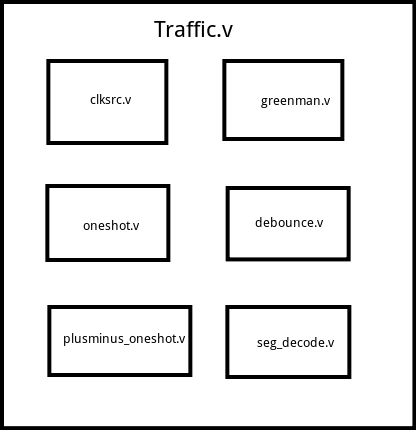
\includegraphics[width=7cm]{block}
  \caption{系統區塊圖}
\end{figure}
\begin{itemize}
\item clksrc: phase lock loop模組。
\item greenman.v: 控制小綠人的模組。
\item seg\_decode.v: 控制七段顯示器的模組。
\item oneshot.v: 處理控制next按鈕訊號的模組。
\item plusminus\_oneshot.v: 處理控制加減秒數和reset按鈕訊號的模組。
\item debounce.v: 將按鈕訊號debounce。
\end{itemize}
\section{狀態}
\begin{figure}[H]
  \centering
  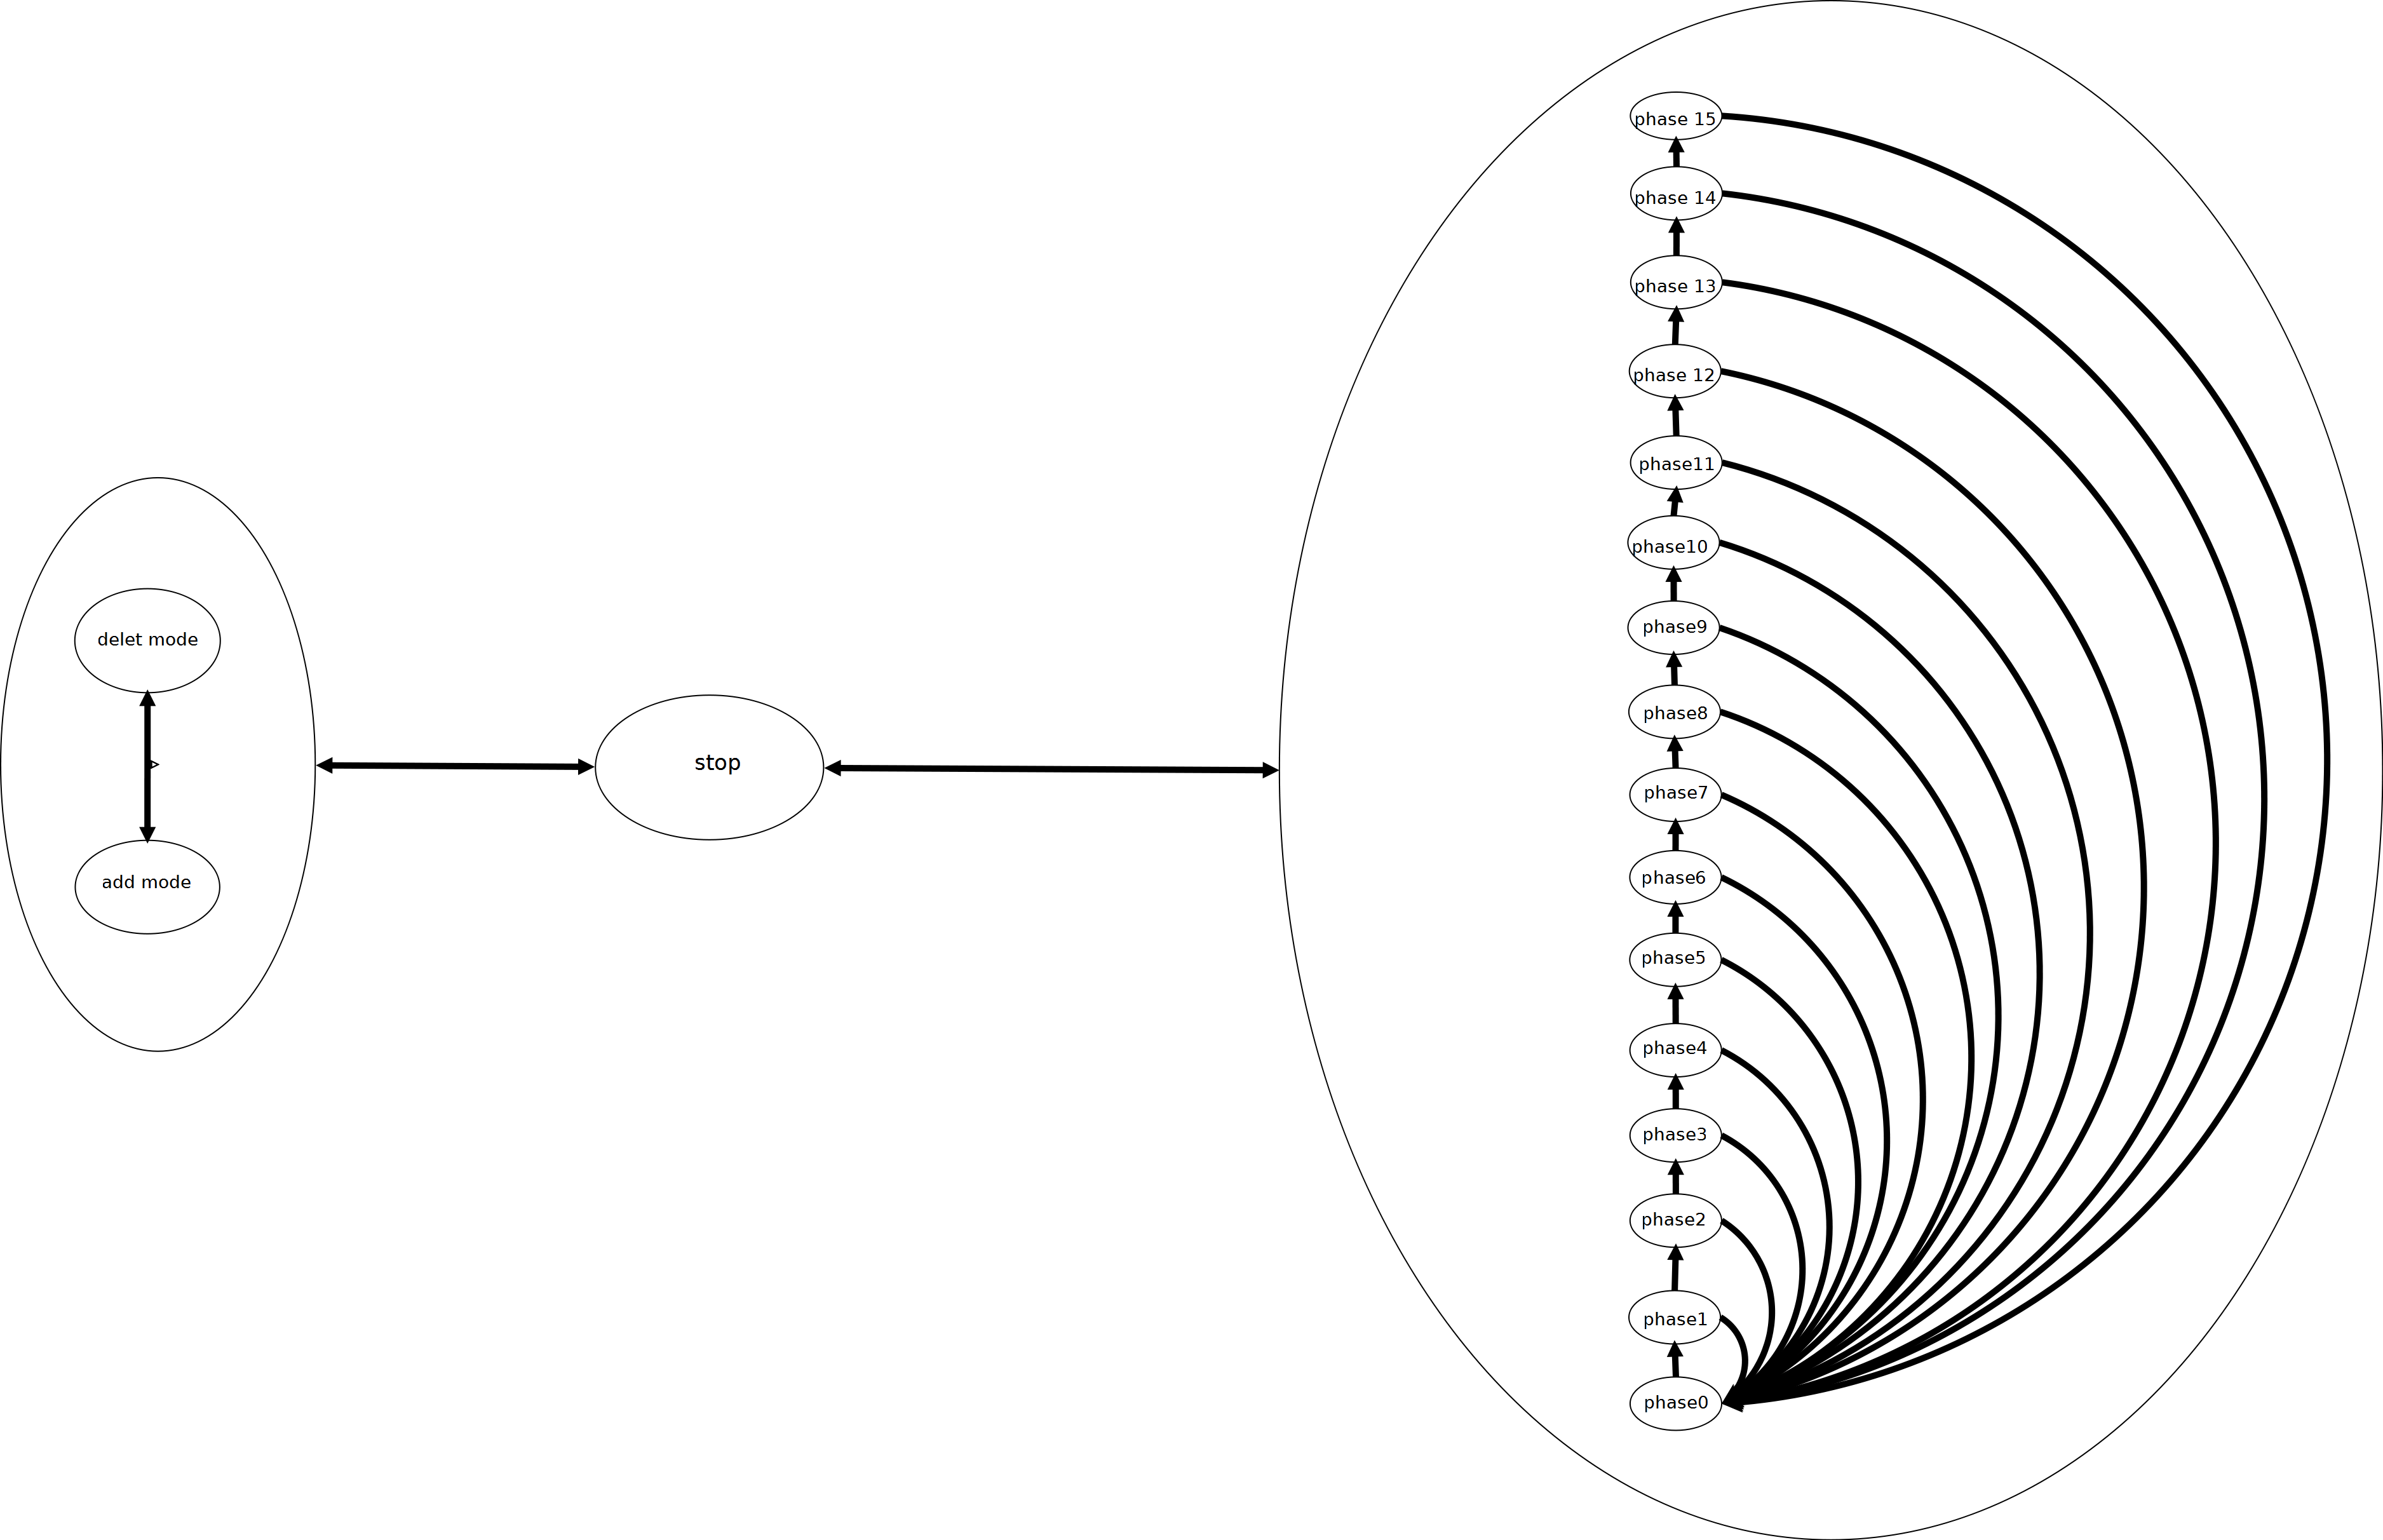
\includegraphics[width=18cm]{state}
  \caption{State}
\end{figure}
\begin{itemize}
\item Normal mode:每個phase 都含有一組屬於自己的燈號、倒數的時間、及控制小綠人動作的資料,當時間倒數至零時,會向下一個phase移動,當reset啟動時,會由任意phase跳回phase1重新開始。
\item Stop mode:按下stop鈕時進入 Stop mode ,此時可調整該phase倒數的時間。
\item Add mode:在Stop mode時add鈕向上撥進入Add mode,此時將插入一個phase,並可編輯該phase的燈號(暗、亮、閃爍)、小綠人動作、倒數的時間。調整完後將add鈕向下扳即回到Stop mode。
\item Delet mode:在Stop mode時delet鈕向上撥即刪掉該phase,向下回到Stop mode。
\end{itemize}

\section{流程}
\begin{figure}[H]
  \centering
  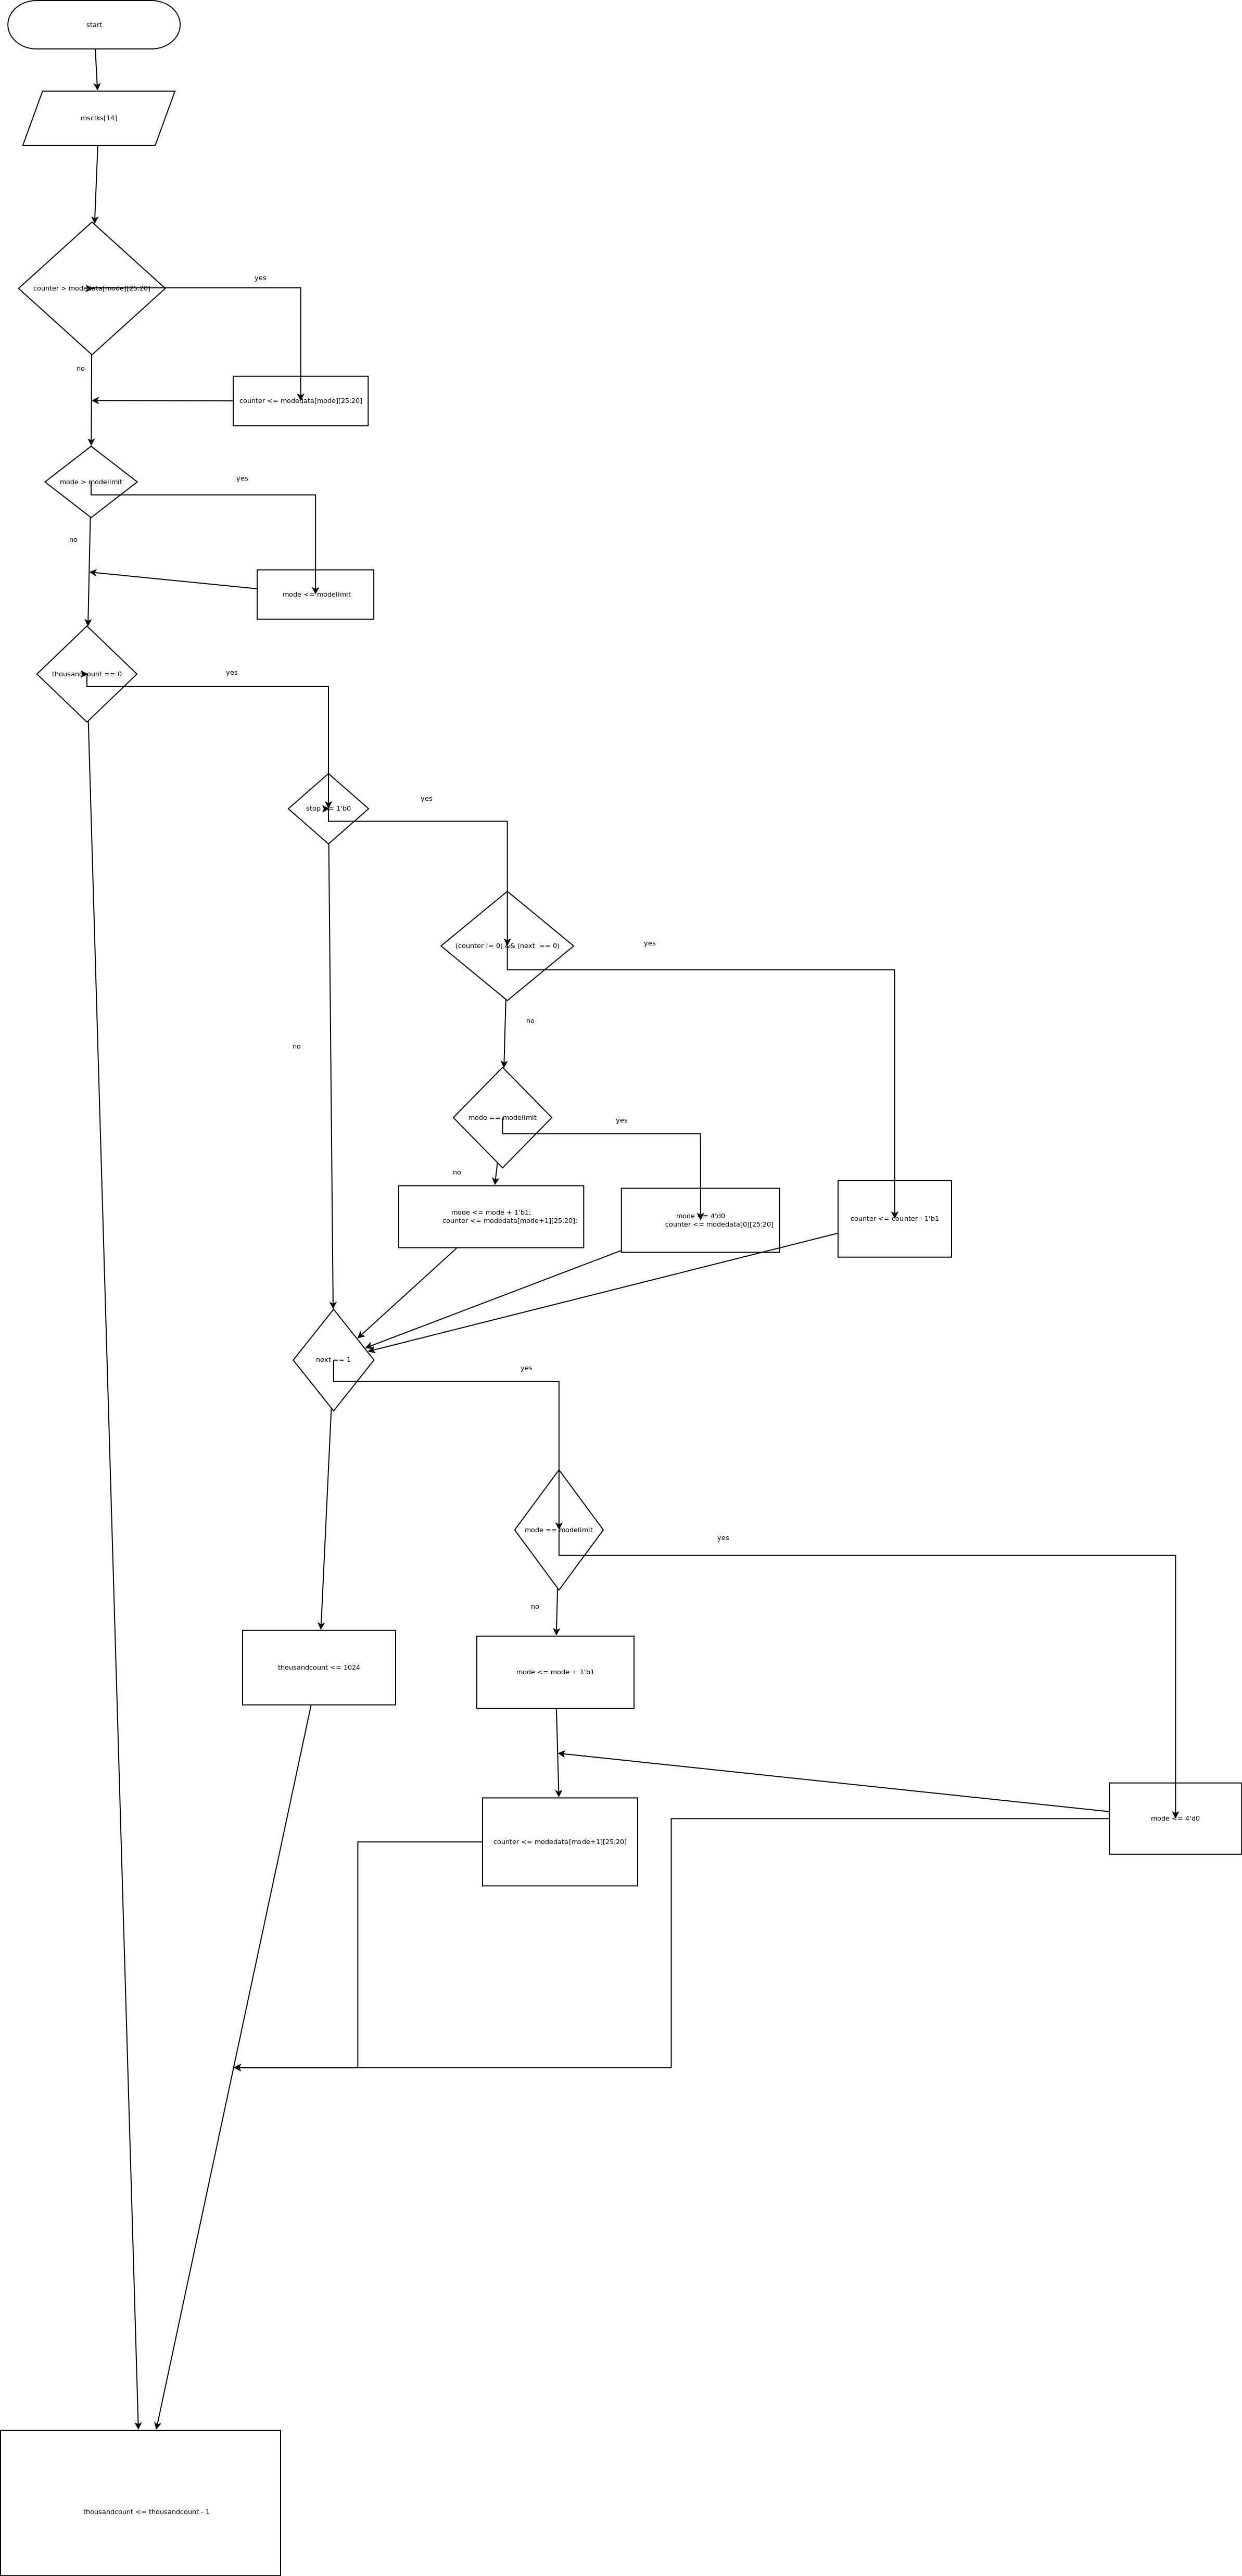
\includegraphics[width=10cm]{control_mode}
  \caption{control mode}
\end{figure}
\begin{figure}[H]
  \centering
  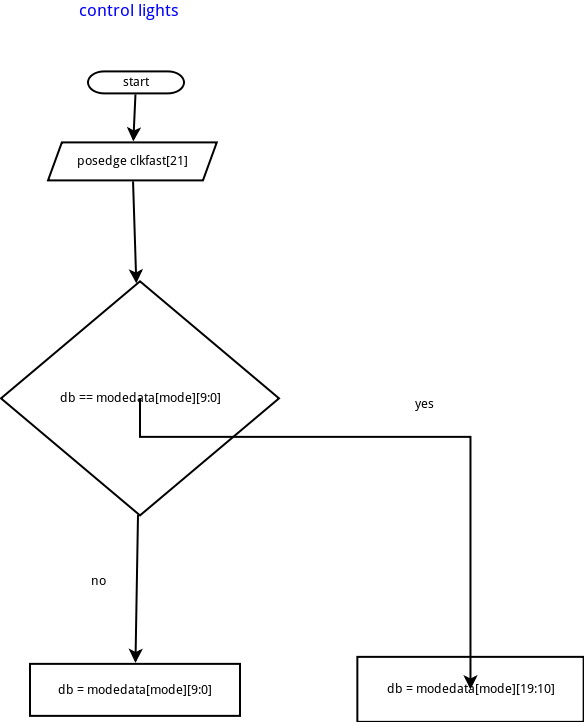
\includegraphics[width=7cm]{lights}
  \caption{control lights}
\end{figure}
\begin{figure}[H]
  \centering
  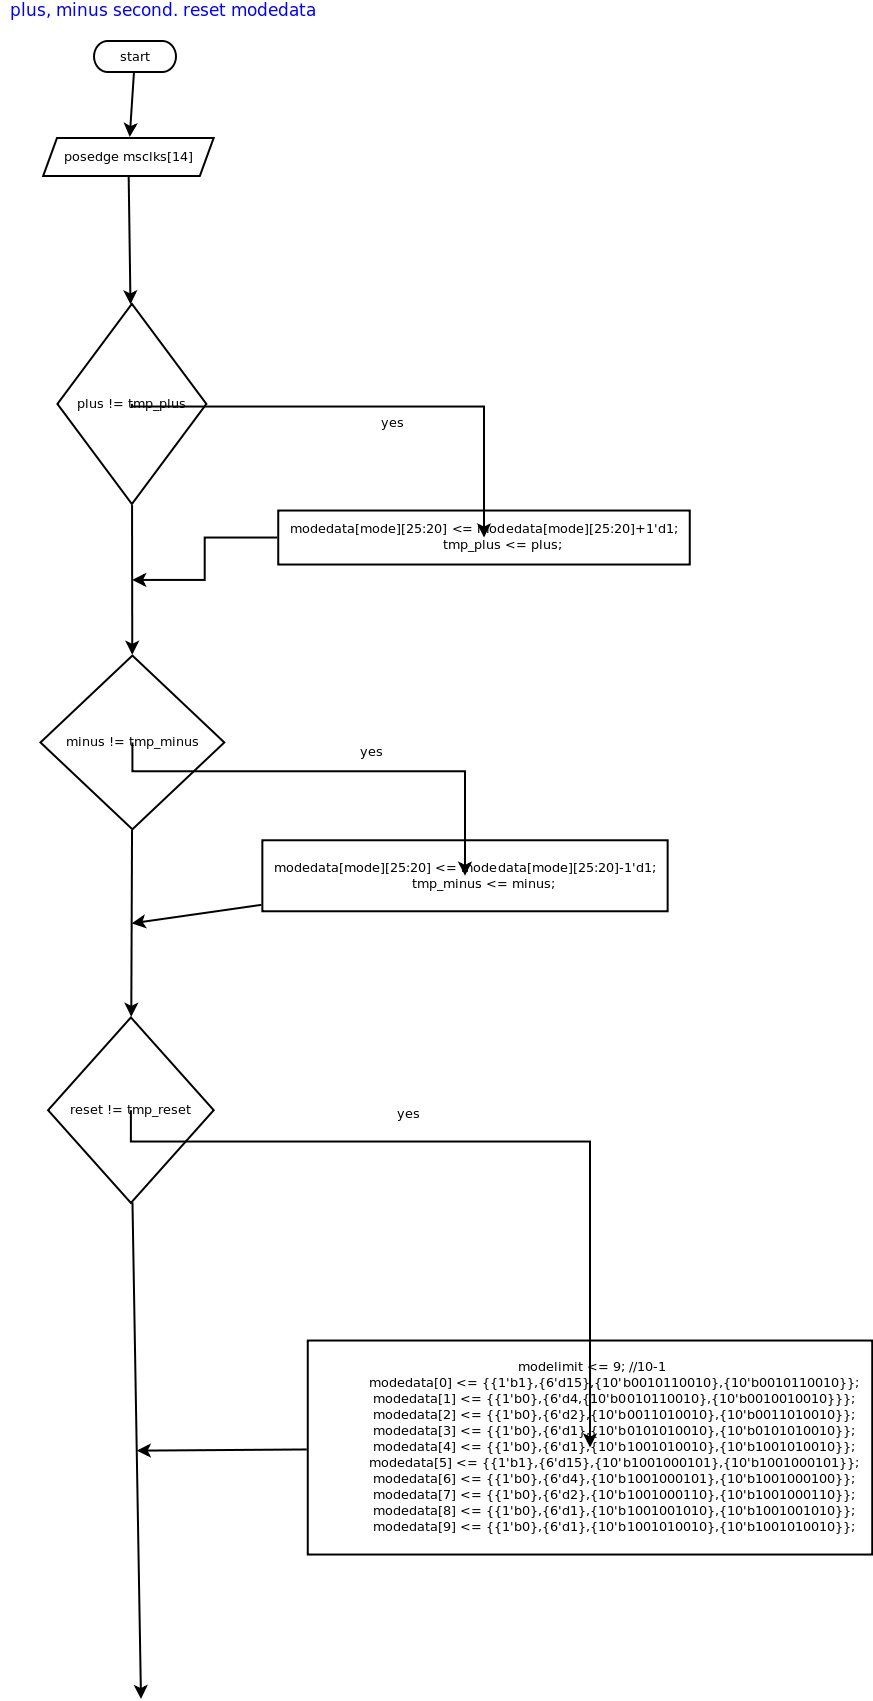
\includegraphics[width=7cm]{plusminus}
  \caption{plus and minus}
\end{figure}
\begin{itemize}
\item control light:控制燈號閃爍
\item control mode :控制燈號狀態是否暫停或跳到下一狀態
\item plus, minus second, reset modedata:控制加減燈號狀態秒數,及設置燈號狀態回初始狀態
\end{itemize}

\end{document}
